%! TEX program = pdflatex

\documentclass[oneside,solution]{karazin-control-assign}

\usepackage[utf8]{inputenc}
\usepackage[english,ukrainian]{babel}

\title{Контрольна Робота}
\author{Захаров Дмитро}
\studentID{МП-31}
\instructor{Сморцова Т.І.}
\date{\today}
\duedate{23:59 14 травня, 2024}
\assignno{1}
\semester{Весняний семестр 2024}
\mainproblem{Варіант 4}

\begin{document}

\maketitle

% \startsolution[print]

\problem{Трикутна система}

\hspace{20px}\textbf{Умова.} Знайти керування, яке переводить точку $(0,-1,-1)$ в точку $(0,0,0)$ в силу системи
\begin{equation}
    \begin{cases}
        \dot{x}_1 = e^{x_1} + x_2 - 1 \\
        \dot{x}_2 = -x_2e^{x_1} + x_3 \\
        \dot{x}_3 = -2e^{3x_1} - (x_2-3)e^{2x_1} - e^{x_1} + u
    \end{cases}
\end{equation}

за проміжок часу $[0,2]$. Виписати траєкторію системи, за якою відбувається цей перехід. Знайти керування, яке стабілізує задану систему.

\textbf{Розв'язання.} Помітимо, що наша система є трикутною, тобто її можна записати у вигляді
\begin{equation}
    \begin{cases}
        \dot{x}_1 = f_1(x_1,x_2) \\
        \dot{x}_2 = f_2(x_1,x_2,x_3) \\
        \dot{x}_3 = f_3(x_1,x_2,x_3,u)
    \end{cases},
\end{equation}

де $f_1(x_1,x_2)=e^{x_1}+x_2-1,f_2(x_1,x_2,x_3)=-x_2e^{x_1}+x_3$ та $f_3(x_1,x_2,x_3,u)=-2e^{3x_1}-(x_2-3)e^{2x_1} - e^{x_1} + u$. 

Скористаємося \textit{теоремою Коробова (про керованість трикутних систем)}. Знайдемо наступні похідні:
\begin{gather}
    \frac{\partial f_1}{\partial x_2} = \frac{\partial f_2}{\partial x_3} = \frac{\partial f_3}{\partial u} = 1 > 0
\end{gather}

Отже, за теоремою (оскільки $\left|\partial f_i/\partial x_{i+1}\right| \geq 1 > 0 \; \forall i \in \{1,\dots,n\}$) робимо висновок, що система є повністю керованою на $[0,2]$. 

Отже, зробимо наступну заміну змінних:
\begin{gather}
    z_1 = x_1, \; z_2 = f_1(x_1,x_2), \nonumber \\ z_3 = \frac{\partial f_1}{\partial x_1}\cdot f_1(x_1,x_2) + \frac{\partial f_1}{\partial x_2}\cdot f_2(x_1,x_2,x_3)
\end{gather}

Якщо підставити вирази для $f_i, i \in \{1,2,3\}$:
\begin{gather}
    z_1 = F_1(x_1) = x_1, \; z_2 = F_2(x_1,x_2) = e^{x_1}+x_2-1, \nonumber \\ z_3 = F_3(x_1,x_2,x_3) =  e^{x_1}(e^{x_1}+x_2-1) + (-x_2e^{x_1} + x_3) = e^{2x_1} - e^{x_1} + x_3
\end{gather}

Нарешті, замінимо керування наступним чином:
\begin{gather}
    v := F_4(x_1,x_2,x_3,u) = \frac{\partial F_3}{\partial x_1}f_1(x_1,x_2) + \frac{\partial F_3}{\partial x_2}f_2(x_1,x_2,x_3) + \frac{\partial F_3}{\partial x_3}f_3(x_1,x_2,x_3,u) \nonumber\\
    = (2e^{2x_1} - e^{x_1})(e^{x_1}+x_2-1) - 2e^{3x_1} - (x_2 - 3)e^{2x_1} - e^{x_1} + u \nonumber \\
    = u + e^{x_1}(e^{x_1}-1)x_2
\end{gather}

Тепер підсумуємо все, що ми нарахували:
\begin{equation}\label{zam}
    \begin{cases}
        z_1 = x_1 \\
        z_2 = e^{x_1} + x_2 - 1 \\
        z_3 = e^{2x_1} - e^{x_1} + x_3 \\
        v = x_2e^{x_1}(e^{x_1}-1) + u
    \end{cases}
\end{equation}

Отже помітимо, що ми таким чином звели систему до вигляду:
\begin{equation}\label{eq:1}
    \begin{cases}
        \dot{z}_1 = z_2 \\
        \dot{z}_2 = z_3 \\
        \dot{z}_3 = v
    \end{cases}
\end{equation}

З такою системою працювати значно приємніше, оскільки тепер нам треба перевести точку $\mathbf{z}(0)$ у $\mathbf{z}(2)$ за допомогою керування $v$. Знайдемо самі координати:
\begin{equation}
    \mathbf{z}(0) = \begin{bmatrix}
        F_1(0) \\
        F_2(0,-1) \\
        F_3(0,-1,-1)
    \end{bmatrix} = \begin{bmatrix}
        0 \\ -1 \\ -1
    \end{bmatrix}, \; \mathbf{z}(2) = \begin{bmatrix}
        F_1(0) \\
        F_2(0,0) \\
        F_3(0,0,0)
    \end{bmatrix} = \begin{bmatrix}
        0 \\ 0 \\ 0
    \end{bmatrix}
\end{equation}

Цікаво, що вони збіглися з початковими. Таким чином, переводимо точку $(0,-1,-1)$ у $(0,0,0)$ за час $T=2$ в силу системи \ref{eq:1}. Можемо її записати у вигляді:
\begin{equation}
    \dot{\mathbf{z}} = \boldsymbol{A}\mathbf{z}(t) + \boldsymbol{\beta}v, \; \boldsymbol{A} = \begin{bmatrix}
        0 & 1 & 0 \\
        0 & 0 & 1 \\
        0 & 0 & 0
    \end{bmatrix}, \; \boldsymbol{\beta} = \begin{bmatrix}
        0 \\ 0 \\ 1
    \end{bmatrix}
\end{equation}

Матрична експонента:
\begin{equation}
    \exp(-\mathbf{A}t) = \begin{bmatrix}
        1 & -t & \frac{t^2}{2} \\
        0 & 1 & -t \\
        0 & 0 & 1
    \end{bmatrix}, \; \mathbf{w}(t) := \exp(-\mathbf{A}t)\boldsymbol{\beta} = \begin{bmatrix}
        \frac{t^2}{2} \\ -t \\ 1
    \end{bmatrix}
\end{equation}

Знаходимо матрицю керованості:
\begin{equation}
    \boldsymbol{N}(0,2) = \int_0^2 \mathbf{w}(t)\mathbf{w}^{\top}(t)dt = \int_0^2\begin{bmatrix}
        \frac{t^4}{4} & -\frac{t^3}{2} & \frac{t^2}{2} \\
        -\frac{t^3}{2} & t^2 & -t \\
        \frac{t^2}{2} & -t & 1
    \end{bmatrix}dt = \begin{bmatrix}
        \frac{8}{5} & -2 & \frac{4}{3} \\
        -2 & \frac{8}{3} & -2 \\
        \frac{4}{3} & -2 & 2
    \end{bmatrix}
\end{equation}

Беремо обернену матрицю:
\begin{equation}
    \boldsymbol{N}^{-1}(0,2) = \begin{bmatrix}
        \frac{8}{5} & -2 & \frac{4}{3} \\
        -2 & \frac{8}{3} & -2 \\
        \frac{4}{3} & -2 & 2
    \end{bmatrix}^{-1} = \begin{bmatrix}
        \frac{45}{2} & \frac{45}{2} & \frac{15}{2} \\
        \frac{45}{2} & 24 & 9 \\
        \frac{15}{2} & 9 & \frac{9}{2}
    \end{bmatrix}
\end{equation}

Нарешті, керування можна знайти як:
\begin{equation}
    v(t) = \boldsymbol{\beta}^{\top}e^{-\boldsymbol{A}^{\top}t}\boldsymbol{N}^{-1}(0,2)\left(\mathbf{0} - e^{-\boldsymbol{A} \cdot 0}\begin{bmatrix}
        0 \\ -1 \\ -1
    \end{bmatrix}\right)
\end{equation}

Підставляючи, маємо:
\begin{equation}
    v(t) = -\begin{bmatrix}
        \frac{t^2}{2} & -t & 1
    \end{bmatrix}\begin{bmatrix}
        \frac{45}{2} & \frac{45}{2} & \frac{15}{2} \\
        \frac{45}{2} & 24 & 9 \\
        \frac{15}{2} & 9 & \frac{9}{2}
    \end{bmatrix}\begin{bmatrix}
        0 \\ -1 \\ -1
    \end{bmatrix} = 15t^2 - 33t + \frac{27}{2},
\end{equation}

Позначимо через $Q_v(t) := 15t^2-33t+\frac{27}{2}$ (далі це буде зручно). Перевіримо, що це дійсно правильне керування. Якщо розв'язати \ref{eq:1}, врахувавши початкову умову $\mathbf{z}(0)=(0,-1,-1)$, отримаємо:
\begin{equation}
    \begin{cases}
        z_1(t) = \frac{2t^5-11t^4+18t^3-4t^2-8t}{8} = Q_1(t) \\
        z_2(t) = \frac{5t^4 - 22t^3 + 27t^2 - 4t - 4}{4} = Q_2(t) \\
        z_3(t) = \frac{10t^3 - 33t^2 + 27t - 2}{2} = Q_3(t)
    \end{cases},
\end{equation}

де ми позначили поліномами $Q_1(t),Q_2(t),Q_3(t)$ ті страшнуваті вирази, що ми знайшли. Далі все будемо виражати через них. 

Можна дійсно переконатись, що $z_1(2)=z_2(2)=z_3(2)=0$, а отже керування правильне. Отже, залишилось знайти $x_1(t),x_2(t),x_3(t)$ та $u(t)$, маючи $z_i(t)$ та $v(t)$. 

Отже, для початку $x_1(t)=z_1(t) = Q_1(t)$. Далі, помічаємо, що
\begin{equation}
    z_2 = e^{x_1}+x_2-1 \implies x_2(t) = Q_2(t) - e^{Q_1(t)} + 1
\end{equation}

Далі для $x_3$:
\begin{equation}
    z_3 = e^{2x_1} - e^{x_1} + x_3 \implies x_3(t) = Q_3(t) - e^{2Q_1(t)} + e^{Q_1(t)}
\end{equation}

Нарешті, щоб знайти керування $u(t)$, помічаємо:
\begin{equation}
    v = u + e^{x_1}(e^{x_1}-1)x_2 \implies u(t) = Q_v(t) - Q_2(t)e^{Q_1(t)}(e^{Q_1(t)}-1)
\end{equation}

Отже, \textbf{відповідь на перше питання}: шукане керування має вигляд $u(t) = Q_v(t) - Q_2(t)e^{Q_1(t)}(e^{Q_1(t)}-1)$, котре задає траєкторію системи:
\begin{equation}
    \mathbf{x}(t) = (Q_1(t), Q_2(t) - e^{Q_1(t)}+1, Q_3(t) - e^{2Q_1(t)}+e^{Q_1(t)}),
\end{equation}
де через $Q_1,Q_2,Q_3,Q_v$ ми позначили наступні поліноми від $t$:
\begin{gather}
    Q_1(t) = \frac{2t^5-11t^4+18t^3-4t^2-8t}{8}, \; Q_2(t) = \frac{5t^4-22t^3+27t^2-4t-4}{4}, \nonumber \\ Q_3(t) = \frac{10t^3-33t^2+27t-2}{2}, \; Q_v(t) = 15t^2 - 33t + \frac{27}{2}
\end{gather}

Побудовану траєкторію можна побачити на Рисунку \ref{fig:problem_1}.

\begin{figure}
    \centering
    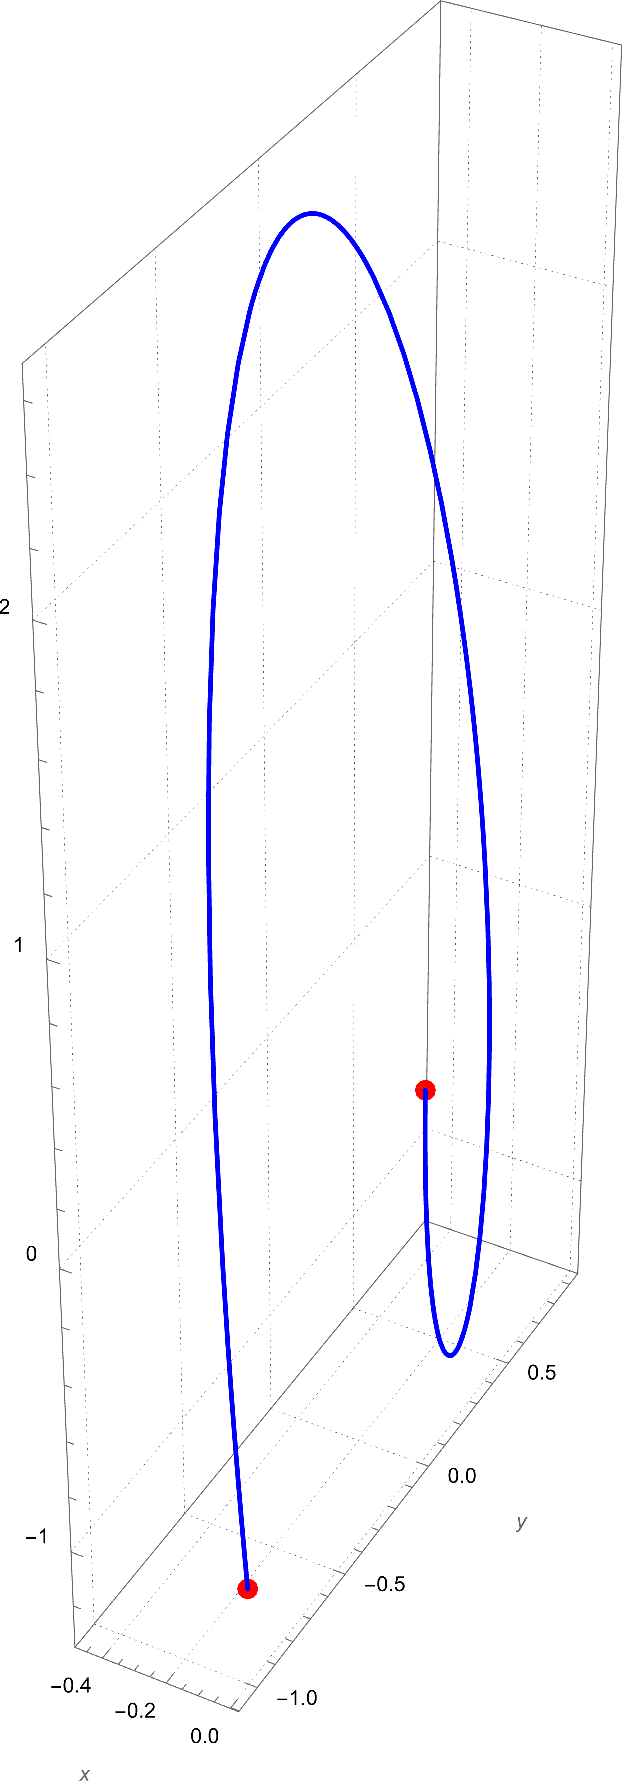
\includegraphics[width=0.5\textwidth]{test_3_problem_1.pdf}
    \caption{Графік траєкторії з задачі 1 для керування $u(t) = Q_v(t) - Q_2(t)e^{Q_1(t)}(e^{Q_1(t)}-1)$}
    \label{fig:problem_1}
\end{figure}

\textbf{Стабілізація.} Бачимо, що $f_i(\mathbf{0})=0$, а отже за теоремою Коробова існує стабілізаційне керування. Щоб стабілізувати нашу вхідну систему, стабілізуємо систему \ref{eq:1}. Для цього будемо шукати керування у вигляді $v=p_1z_1+p_2z_2+p_3z_3$. Тоді отримаємо систему:
\begin{equation}
    \dot{\mathbf{z}} = \begin{bmatrix}
        0 & 1 & 0 \\
        0 & 0 & 1 \\
        p_1 & p_2 & p_3
    \end{bmatrix}\mathbf{z}
\end{equation}

Нам потрібно, щоб усі власні значення цієї матриці лежали у лівій напівплощині $\text{Re}(z) < 0$. Отже, знаходимо характеристичний поліном:
\begin{equation}
    \chi(\lambda) = \det\begin{bmatrix}
        -\lambda & 1 & 0 \\
        0 & -\lambda & 1 \\
        p_1 & p_2 & p_3-\lambda
    \end{bmatrix} = -\lambda^3 + p_3\lambda^2 + p_2\lambda + p_1
\end{equation}

Підберемо $(p_1,p_2,p_3)$ таким чином, щоб усі корені мали від'ємну дійсну частину. Наприклад, нехай $\chi(\lambda)=-(\lambda+1)^3$, тоді $p_1=-1,p_2=-3,p_3=-3$. В такому разі, маємо одне власне число $\lambda=-1$ кратності 3 і тому керування $v=-z_1-3z_2-3z_3$ стабілізує нашу систему. Повернемось до $u$:
\begin{equation}
    u = v - x_2e^{x_1}(e^{x_1}-1) = -z_1-3z_2-3z_3 - x_2e^{x_1}(e^{x_1}-1)
\end{equation}

Отже, залишається лише скористатись заміною \ref{zam} аби записати $u$ як функцію від координат $x_1,x_2,x_3$. Отримуємо
\begin{equation}
    \boxed{u(x_1,x_2,x_3) = x_2e^{x_1} - e^{2x_1}(x_2+3) - x_1 - 3x_2 - 3x_3 + 3}
\end{equation}

\problem{Кусково-стале керування}

\hspace{20px}\textbf{Умова.} Знайти кусково-стале керування, яке переводить точку $(-1,1)$ в точку $(0,0)$ в силу системи
\begin{equation}
    \begin{cases}
        \dot{x} = x^4 + y \\
        \dot{y} = -4x^7 - 4x^3y + u
    \end{cases}
\end{equation}

за проміжок часу $[0,4]$ та має перемикання в точці $t_1=2$.

\textbf{Розв'язання.} Зробимо заміну $z_1=x, z_2=x^4+y$ і заміну керування
\begin{equation}
    v = 4x^3(x^4+y) + (-4x^7 - 4x^3y + u) = u
\end{equation}

Тоді, наша початкова система перейде у
\begin{equation}\label{eq:2_1}
    \begin{cases}
        \dot{z}_1 = z_2 \\
        \dot{z}_2 = u
    \end{cases}
\end{equation}

Початкова точка перейде у $(-1,2)$, а кінцева у $(0,0)$. Таким чином, потрібно за проміжок часу $[0,4]$ перевести точку $(-1,2)$ у $(0,0)$ в силу системи \ref{eq:2_1}. Як і сказано в умові, шукаємо керування у вигляді
\begin{equation}
    u(t) = \begin{cases}
        \alpha, & t \in [0, 2] \\
        \beta, & t \in (2, 4]
    \end{cases}
\end{equation}

В такому разі, на відрізку $[0,2]$ $z_2=\alpha t + b$. Оскільки $z_2(0) = 2$, то $b=2$, а тому $z_2(t)=\alpha t + 2$. Тому $z_1 = \frac{\alpha t^2}{2} + 2t + c$. Оскільки $z_1(0)=-1$, то $c=-1$ і тому $z_1(t) = \frac{\alpha t^2}{2} + 2t - 1$.

Далі розглядаємо проміжок $(2,4]$. Тут $z_2(t) = \beta t + d$. Оскільки $z_2(4)=0$, то $z_2(t) = \beta (t - 4)$. Тому $z_1(t) = \frac{\beta t^2}{2} - 4\beta t + f$. Оскільки $z_1(4)=0$, то $8\beta - 16\beta + f = 0$ і тому $f=8\beta$. Звідси $z_1(t) = \beta\left(\frac{t^2}{2} - 4t + 8\right)$.

Отже, залишилось знайти $\alpha$ та $\beta$. Для цього застосуємо умову неперервності, тобто $\lim_{t \to 2^-}z_i(t) = \lim_{t \to 2^+}z_i(t), \; i \in \{1,2\}$. Отже:
\begin{equation}
    \begin{cases}
    2\beta = 2\alpha + 3 \\
    2\alpha + 2 = -2\beta
    \end{cases}
\end{equation}

Звідси легко отримати $\alpha=-\frac{5}{4},\beta=\frac{1}{4}$. Отже, остаточна відповідь:
\begin{equation}
    u(t) = \begin{cases}
        -\frac{5}{4}, & t \in [0,2] \\
        \frac{1}{4}, & t \in (2,4]
    \end{cases}
\end{equation}

Для самоперевірки впевнимось, що це дійсно правильне керування. Для цього запустимо наступну програму у \textit{Wolfram Mathematica}:

\begin{lstlisting}[language=Mathematica]
u[t_] = Piecewise[{{-(5/4), 0<=t<=2}, {1/4, 2<=t<=4}}, 0];
s = NDSolve[{x'[t] == x[t]^4+y[t], 
    y'[t] == -4*x[t]^7-4*x[t]^3*y[t]+u[t], x[0] == -1, 
    y[0] == 1}, {x, y}, {t, 6}];
ParametricPlot[Evaluate[{x[t], y[t]} /. s], {t, 0, 4}, 
 GridLines -> Automatic, PlotStyle -> {Red, Thickness[0.008]}, 
 AxesLabel -> {x, y}, 
 AxesStyle -> {{14, Arrowheads[0.05]}, {14, Arrowheads[0.05]}}, 
 ImageSize -> 400]
\end{lstlisting}

Результат зображено на Рисунку \ref{fig:problem_2}. Бачимо, що дійсно з точки $(-1,1)$ ми потрапляємо у точку $(0,0)$ за час $T=4$.

\begin{figure}
    \centering
    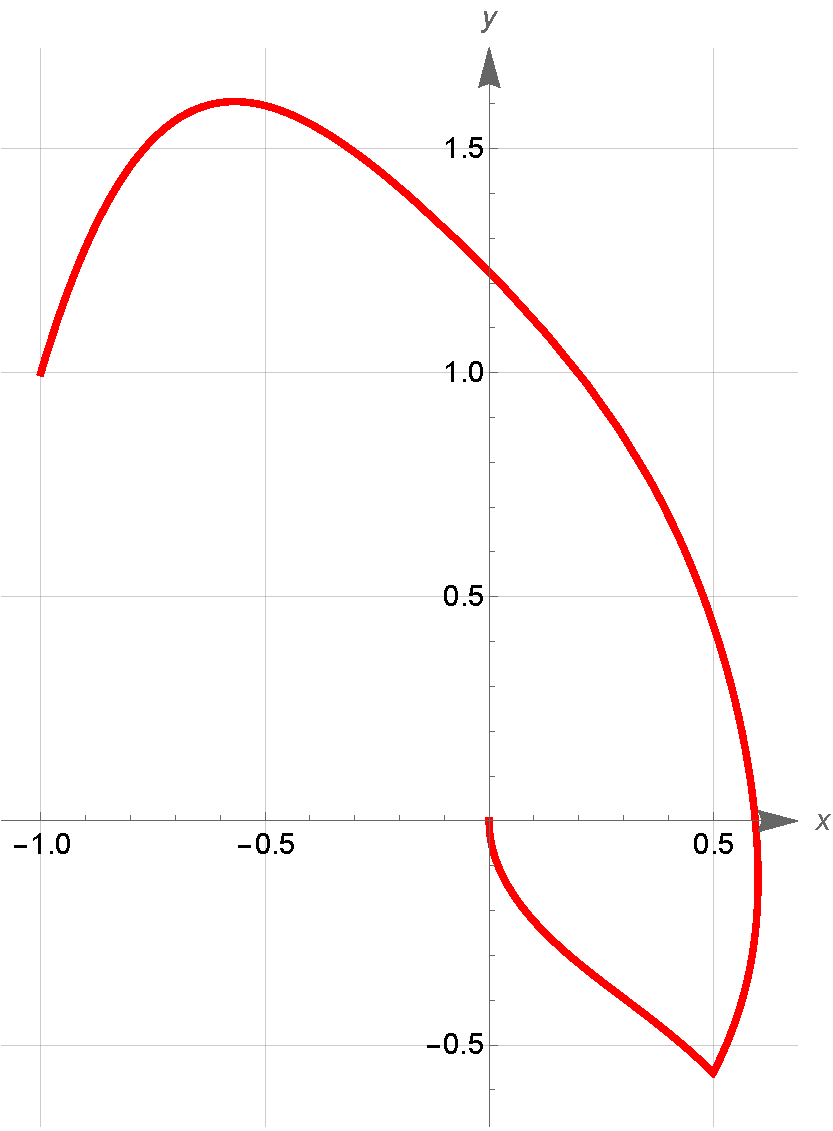
\includegraphics[width=0.6\textwidth]{test_3_problem_2.pdf}
    \caption{Графік траєкторії з задачі 2 для керування $u(t) = \begin{cases}
        -5/4, & t \in [0,2] \\ 1/4, & t \in (2,4]
    \end{cases}$}
    \label{fig:problem_2}
\end{figure}

\end{document}
